\documentclass[12pt,a4paper]{article}

% --- Encodage et langue ---
\usepackage[utf8]{inputenc}
\usepackage[T1]{fontenc}
\usepackage{lmodern}

% --- Maths ---
\usepackage{amsmath,amssymb,amsthm}

% --- Mise en page ---
\usepackage[top=2.5cm,bottom=2.5cm,left=2.8cm,right=2.8cm]{geometry}
\usepackage{parskip}

% --- Tableaux ---
\usepackage{booktabs}
\usepackage{array}
\usepackage{multirow}

% --- Figures et couleurs ---
\usepackage{tikz}
\usetikzlibrary{arrows.meta, positioning, decorations.pathreplacing, calc, fit, backgrounds}
\usepackage{xcolor}

% --- Liens ---
\usepackage{hyperref}
\hypersetup{colorlinks=true, linkcolor=blue!60!black, citecolor=blue!60!black}

% --- Macros (cohérentes avec anatomie_moteur.tex et convergence_sans_bruit.tex) ---
\newcommand{\Inc}{\ensuremath{\mathrm{Include}}}
\newcommand{\Exc}{\ensuremath{\mathrm{Exclude}}}
\newcommand{\vbar}{\bar{v}}
\newcommand{\code}[1]{\texttt{#1}}

% --- Environnement pour les notes/encadrés ---
\theoremstyle{remark}
\newtheorem{note}{Note}[section]
\newtheorem{exemple}{Exemple fil rouge}[section]

% ======================================================
\begin{document}
% ======================================================

\begin{center}
{\LARGE\bfseries Fonctionnement du système}\\[4pt]
{\normalsize Stumps aléatoires + règle à 4 cas, sans routeur}
\end{center}

\begin{figure}[h]
\centering
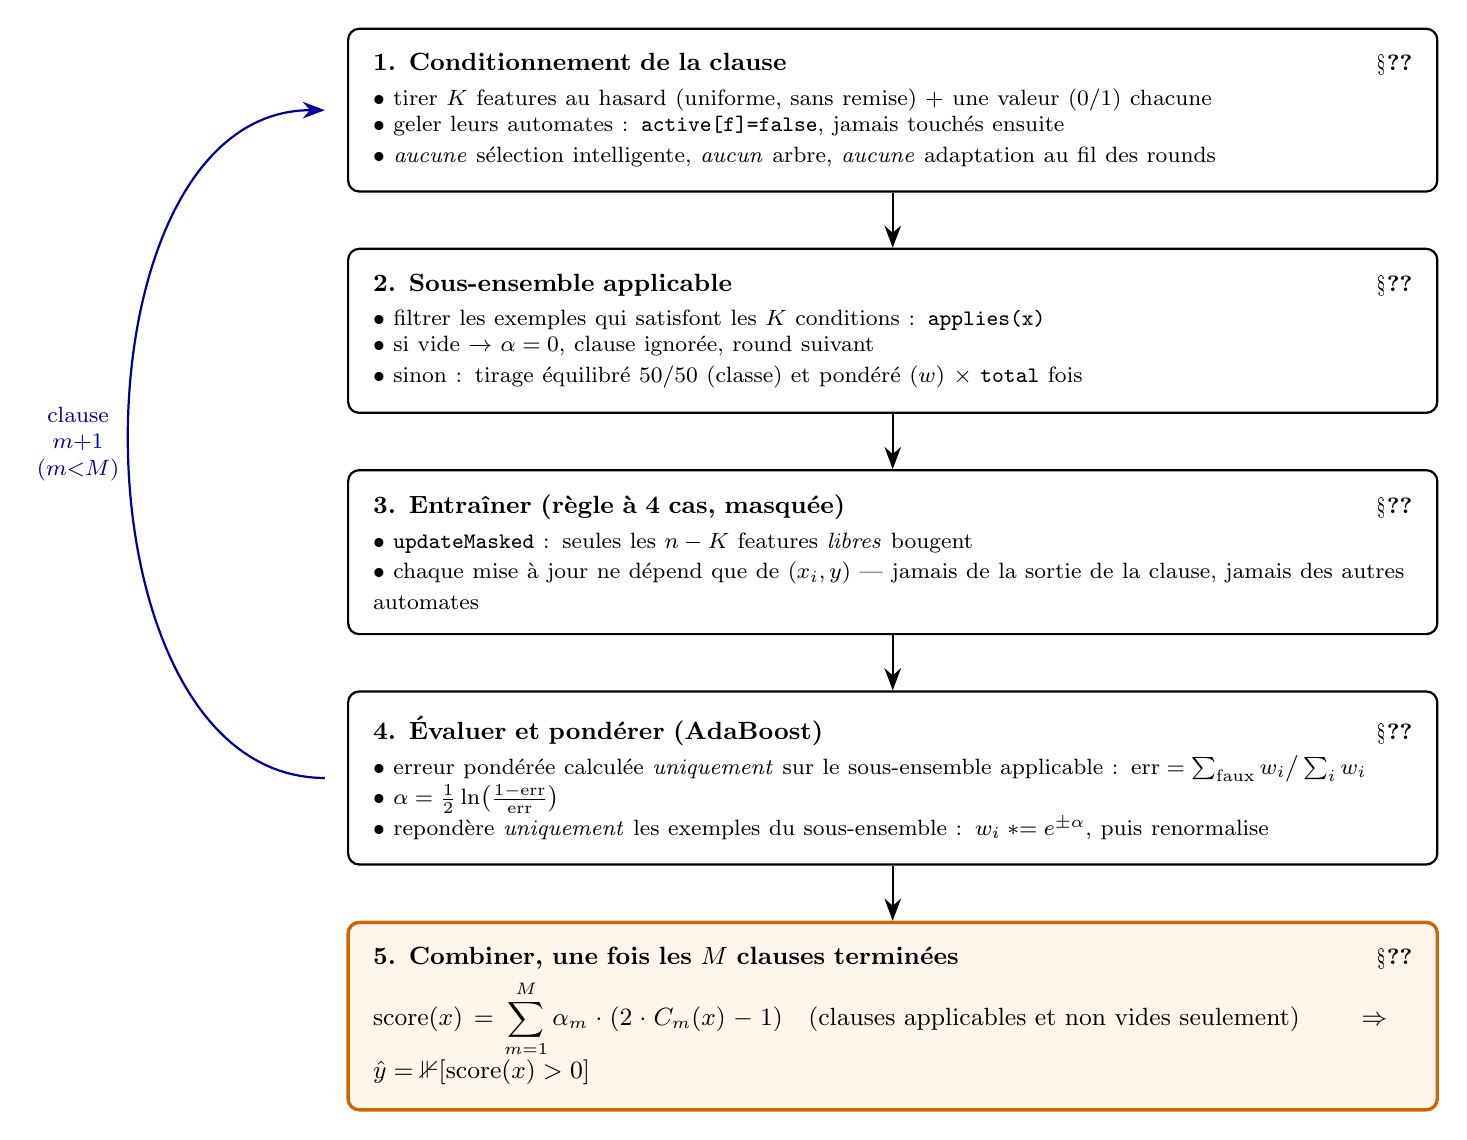
\begin{tikzpicture}[
  bigbox/.style={draw, thick, rounded corners, align=left, font=\small, text width=13.2cm, inner sep=9pt},
  finalbox/.style={draw=orange!80!black, very thick, rounded corners, align=left, font=\small,
                    fill=orange!8, text width=13.2cm, inner sep=9pt},
  arr/.style={-{Stealth[length=8pt]}, thick},
  node distance=0.7cm
]
\node[bigbox] (b1) {\textbf{1. Conditionnement de la clause} \hfill{\footnotesize\S\ref{sec:cond}}\\[3pt]
\footnotesize
$\bullet$ tirer $K$ features au hasard (uniforme, sans remise) $+$ une valeur (0/1) chacune\\
$\bullet$ geler leurs automates : \code{active[f]=false}, jamais touchés ensuite\\
$\bullet$ \emph{aucune} sélection intelligente, \emph{aucun} arbre, \emph{aucune} adaptation au fil des rounds};

\node[bigbox, below=of b1] (b2) {\textbf{2. Sous-ensemble applicable} \hfill{\footnotesize\S\ref{sec:cond}}\\[3pt]
\footnotesize
$\bullet$ filtrer les exemples qui satisfont les $K$ conditions : \code{applies(x)}\\
$\bullet$ si vide $\to$ $\alpha=0$, clause ignorée, round suivant\\
$\bullet$ sinon : tirage équilibré 50/50 (classe) et pondéré ($w$) $\times$ \code{total} fois};

\node[bigbox, below=of b2] (b3) {\textbf{3. Entraîner (règle à 4 cas, masquée)} \hfill{\footnotesize\S\ref{sec:update}}\\[3pt]
\footnotesize
$\bullet$ \code{updateMasked} : seules les $n-K$ features \emph{libres} bougent\\
$\bullet$ chaque mise à jour ne dépend que de $(x_i,y)$ --- jamais de la sortie de la clause,
jamais des autres automates};

\node[bigbox, below=of b3] (b4) {\textbf{4. Évaluer et pondérer (AdaBoost)} \hfill{\footnotesize\S\ref{sec:boost}}\\[3pt]
\footnotesize
$\bullet$ erreur pondérée calculée \emph{uniquement} sur le sous-ensemble applicable :
$\mathrm{err}=\sum_{\text{faux}} w_i \big/ \sum_i w_i$\\
$\bullet$ $\alpha=\tfrac12\ln\!\big(\tfrac{1-\mathrm{err}}{\mathrm{err}}\big)$\\
$\bullet$ repondère \emph{uniquement} les exemples du sous-ensemble : $w_i\mathrel{*}=e^{\pm\alpha}$, puis renormalise};

\node[finalbox, below=of b4] (b5) {\textbf{5. Combiner, une fois les $M$ clauses terminées} \hfill{\footnotesize\S\ref{sec:combine}}\\[3pt]
$\mathrm{score}(x)=\displaystyle\sum_{m=1}^{M}\alpha_m\cdot(2\cdot C_m(x)-1)
\quad\text{(clauses applicables et non vides seulement)}\qquad \Rightarrow\qquad \hat y = \mathbb{1}[\mathrm{score}(x)>0]$};

\draw[arr] (b1) -- (b2);
\draw[arr] (b2) -- (b3);
\draw[arr] (b3) -- (b4);
\draw[arr] (b4) -- (b5);
\draw[arr, blue!60!black] ([xshift=-8pt]b4.west) to[out=180,in=180]
  node[left,font=\footnotesize,text=blue!60!black,align=center]{clause\\$m{+}1$\\($m{<}M$)} ([xshift=-8pt]b1.west);
\end{tikzpicture}
\caption{Vue d'ensemble complète : chaque clause $m=1,\dots,M$ est un round
AdaBoost \textbf{totalement indépendant} des autres --- aucune étape ne
nécessite de connaître l'état d'une autre clause. C'est la différence
structurelle centrale avec la vraie Tsetlin Machine (feedback Type I/II,
couplage via la somme globale des clauses) et avec notre ancienne architecture
à routeur (voir \emph{anatomie\_moteur.tex}) : ici, \textbf{aucun routeur, à
aucun niveau}.}
\label{fig:master-overview}
\end{figure}

% ======================================================
\section{Le trajet d'un exemple, du dataset à la sortie}
% ======================================================

On utilise partout dans ce document le même petit dataset jouet : $n=4$
features booléennes $x=(x_0,x_1,x_2,x_3)$, une étiquette $y\in\{0,1\}$, et une
clause déjà créée avec $K=2$ features conditionnées, tirées au hasard :
$\{0,2\}$, fixées respectivement à $(1,1)$.

\begin{center}
\renewcommand{\arraystretch}{1.25}
\begin{tabular}{lc}
\toprule
 & \textbf{clause (exemple fil rouge)} \\
\midrule
features conditionnées ($K=2$) & $\{0,2\}$, fixées à $(1,1)$ \\
features libres ($n-K=2$)      & $\{1,3\}$ \\
condition \code{applies(x)}    & vraie ssi $x_0{=}1$ et $x_2{=}1$ \\
\bottomrule
\end{tabular}
\end{center}

\noindent Contrairement à l'ancienne architecture à routeur, \textbf{aucun
calcul de gain, aucune structure partagée} ne détermine ce choix : $\{0,2\}$ et
leurs valeurs sont un tirage \code{uniform\_int\_distribution} pur, indépendant
de toute autre clause déjà créée.

Voici tout le trajet d'un exemple à travers cette clause \emph{déjà
entraînée}. Une clause, c'est : une condition figée sur $K$ features
(section~\ref{sec:cond}) qui décide si la clause s'applique du tout à cet
exemple, et un simple \textbf{ET logique} de littéraux appris sur les $n-K$
features libres (section~\ref{sec:update}).

\begin{exemple}
On prend $x=(1,1,1,0)$. La condition de la clause fil rouge teste
$x_0{=}1$ (vrai) et $x_2{=}1$ (vrai) : la clause \textbf{s'applique}.
Supposons qu'elle ait appris, sur ses deux features libres $\{1,3\}$ :
$v[1]=\Inc$ (le littéral ``$x_1$'') et $\vbar[3]=\Inc$ (le littéral
``$\neg x_3$''), tout le reste exclu.
\end{exemple}

\begin{figure}[h]
\centering
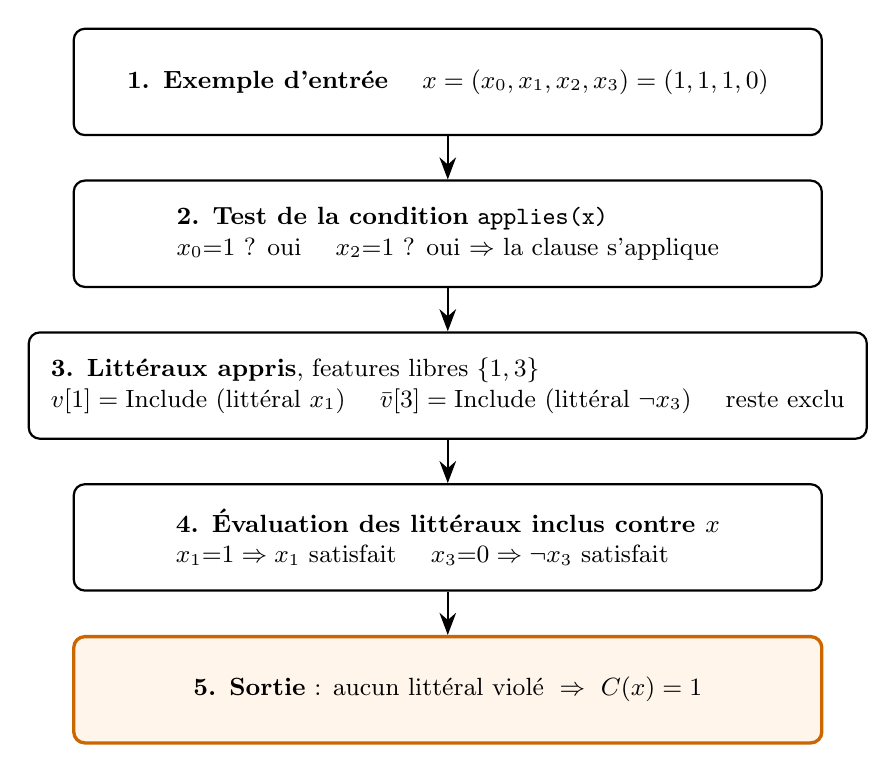
\begin{tikzpicture}[
  stage/.style={draw, rounded corners, thick, minimum width=9.5cm, minimum height=1.35cm,
                align=left, font=\small, inner sep=8pt},
  final/.style={stage, draw=orange!80!black, very thick, fill=orange!8, align=center},
  arr/.style={-{Stealth[length=8pt]}, thick},
  node distance=0.55cm
]
\node[stage, align=center] (s1) {\textbf{1. Exemple d'entrée} $\quad x=(x_0,x_1,x_2,x_3)=(1,1,1,0)$};
\node[stage, below=of s1] (s2) {\textbf{2. Test de la condition} \code{applies(x)}\\
  $x_0{=}1$ ? oui \quad $x_2{=}1$ ? oui $\Rightarrow$ la clause s'applique};
\node[stage, below=of s2] (s3) {\textbf{3. Littéraux appris}, features libres $\{1,3\}$\\
  $v[1]=\Inc$ (littéral $x_1$) \quad $\vbar[3]=\Inc$ (littéral $\neg x_3$) \quad reste exclu};
\node[stage, below=of s3] (s4) {\textbf{4. Évaluation des littéraux inclus contre $x$}\\
  $x_1{=}1\Rightarrow x_1$ satisfait \quad $x_3{=}0\Rightarrow \neg x_3$ satisfait};
\node[final, below=of s4] (s5) {\textbf{5. Sortie} : aucun littéral violé
  $\;\Rightarrow\;$ $C(x)=1$};

\draw[arr] (s1) -- (s2);
\draw[arr] (s2) -- (s3);
\draw[arr] (s3) -- (s4);
\draw[arr] (s4) -- (s5);
\end{tikzpicture}
\caption{Le trajet complet d'un exemple, du dataset à la sortie d'une clause.
Si \code{applies(x)} avait été fausse à l'étape 2, la clause se serait
\textbf{abstenue} : ni entraînement, ni vote, pour cet exemple précis.}
\label{fig:pipeline-inference}
\end{figure}

\subsection{Que veut dire ``littéral inclus'' ?}

Chaque feature libre $i$ possède deux automates : $v[i]$ (associé au littéral
$x_i$) et $\vbar[i]$ (associé au littéral $\neg x_i$). Chacun a un état entier
dans $\{1,\dots,2N\}$ : au-dessus de $N$, le littéral est \Inc{} (il compte
dans la clause) ; à $N$ ou en-dessous, il est \Exc{} (il est ignoré). La
clause est le ET logique de tous les littéraux inclus. Elle est
\textbf{violée} dès qu'un seul littéral inclus est faux pour $x$ ; elle est
\textbf{satisfaite} seulement si \emph{tous} ses littéraux inclus sont vrais
pour $x$.

\begin{figure}[h]
\centering
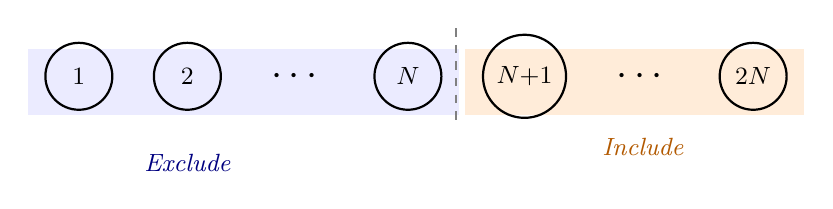
\begin{tikzpicture}[
  state/.style={circle, draw=black, thick, minimum size=0.85cm, font=\small},
  node distance=0.5cm
]
\node[state] (s1) {$1$};
\node[state, right=of s1] (s2) {$2$};
\node[right=0.5cm of s2, font=\Large] (d1) {$\cdots$};
\node[state, right=0.5cm of d1] (sN) {$N$};
\node[state, right=of sN] (sN1) {\small$N{+}1$};
\node[right=0.5cm of sN1, font=\Large] (d2) {$\cdots$};
\node[state, right=0.5cm of d2] (s2N) {$2N$};
\begin{scope}[on background layer]
  \fill[blue!8]  ([xshift=-6pt,yshift=-14pt]s1.west)  rectangle ([xshift=6pt,yshift=10pt]sN.east);
  \fill[orange!15] ([xshift=-6pt,yshift=-14pt]sN1.west) rectangle ([xshift=6pt,yshift=10pt]s2N.east);
\end{scope}
\node[below=12pt of s2, font=\small\itshape, text=blue!50!black] {Exclude};
\node[below=12pt of d2, font=\small\itshape, text=orange!70!black] {Include};
\draw[dashed, gray] ($(sN.north east)+(0.3,0.3)$) -- ($(sN.south east)+(0.3,-0.25)$);
\end{tikzpicture}
\caption{L'état d'un automate se lit sur une seule droite : au-dessus de $N$,
\Inc ; à $N$ ou en-dessous, \Exc. Identique pour les features conditionnées
(figées à l'état $1$, donc toujours \Exc, absentes de la clause) et pour les
features libres (mobiles).}
\label{fig:automate-line}
\end{figure}

% ======================================================
\section{Le conditionnement : un stump aléatoire, pas un routeur}\label{sec:cond}
% ======================================================

C'est le choix architectural central de tout le système. Une approche par
arbre de décision (routeur), même bien conçue, présente une pathologie
prouvée empiriquement : quand $K$ (la profondeur/le nombre de coupures)
devient assez grand, le découpage \emph{seul} devient assez puissant pour
résoudre le problème --- les clauses deviennent décoratives. La solution
retenue : \textbf{éliminer toute adaptation} dans le choix des conditions.

\subsection{Le tirage, à la création de chaque clause}

\begin{figure}[h]
\centering
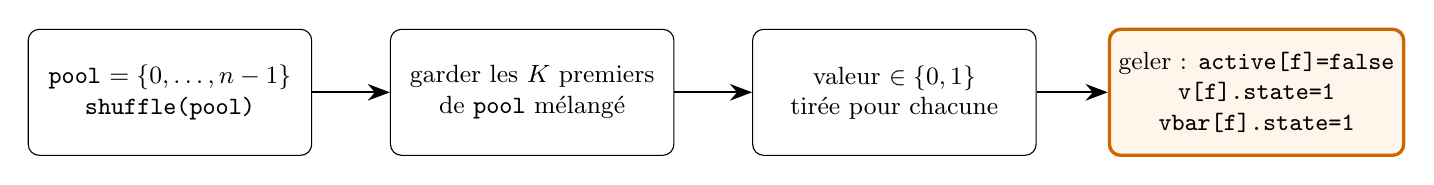
\begin{tikzpicture}[
  cell/.style={draw, rounded corners, minimum width=3.6cm, minimum height=1.6cm, align=center, font=\small},
  arr/.style={-{Stealth[length=8pt]}, thick}
]
\node[cell] (pool) at (0,0) {\code{pool} $=\{0,\dots,n-1\}$\\\code{shuffle(pool)}};
\node[cell] (pick) at (4.6,0) {garder les $K$ premiers\\de \code{pool} mélangé};
\node[cell] (val) at (9.2,0) {valeur $\in\{0,1\}$\\tirée pour chacune};
\node[cell, draw=orange!80!black, very thick, fill=orange!8] (freeze) at (13.8,0)
  {geler : \code{active[f]=false}\\\code{v[f].state=1}\\\code{vbar[f].state=1}};
\draw[arr] (pool) -- (pick);
\draw[arr] (pick) -- (val);
\draw[arr] (val) -- (freeze);
\end{tikzpicture}
\caption{Aucun calcul de gain, aucune information sur $y$ n'intervient dans ce
tirage --- contrairement au routeur de l'ancienne architecture (Gini, gain
$\times$ masse, \emph{anatomie\_moteur.tex} \S\,3), le choix est purement
\code{uniform\_int\_distribution}.}
\label{fig:stump-draw}
\end{figure}

\subsection{La porte d'entrée : \code{applies(x)}}

\[
  \code{applies}(x) = \bigwedge_{k=1}^{K} \big[x_{f_k} = v_k\big]
\]

où $(f_k,v_k)$ sont les $K$ paires (feature, valeur requise) tirées à la
création. Un exemple qui ne satisfait pas \code{applies(x)} est
\textbf{invisible} pour cette clause : ni pour l'entraînement (le
sous-ensemble applicable l'exclut), ni pour le vote final
(section~\ref{sec:combine}).

\begin{note}
Le nombre de combinaisons possibles de $K$ features parmi $n$ est
$\binom{n}{K}$. La probabilité qu'un tirage tombe sur une combinaison
réellement informative décroît donc avec $\binom{n}{K}$ --- c'est la
``loterie combinatoire'' qui impose $M$ (nombre de clauses) grand quand $K>1$
ou $n$ grand (ex.\ Mux11 : $\binom{11}{3}=165$, $M=8000$ nécessaire pour une
couverture correcte des $8$ combinaisons d'adresse).
\end{note}

% ======================================================
\section{Mettre à jour une clause : la règle à 4 cas, masquée}\label{sec:update}
% ======================================================

En dehors des features conditionnées, une clause apprend exactement la règle
à 4 cas démontrée dans \emph{convergence\_sans\_bruit.tex} ---
\code{updateMasked} se contente de sauter les features où
\code{active[i]=false}.

\begin{center}
\renewcommand{\arraystretch}{1.4}
\begin{tabular}{ccll}
\toprule
$x[i]$ & $y$ & Action sur $v[i]$ (littéral $x_i$) & Action sur $\vbar[i]$ (littéral $\neg x_i$) \\
\midrule
0 & 0 & \code{towardInclude}$(S)$   & \code{towardExclude}$(S)$ \\
0 & 1 & \code{towardExclude}$(\alpha)$ & rien \\
1 & 0 & \code{towardExclude}$(S)$   & \code{towardInclude}$(S)$ \\
1 & 1 & rien                      & \code{towardExclude}$(\alpha)$ \\
\bottomrule
\end{tabular}
\end{center}

\begin{exemple}
Reprenons $x=(1,1,1,0)$, applicable à la clause fil rouge, avec $y=1$ (vrai
label). Seules les features libres $\{1,3\}$ sont mises à jour :
\begin{itemize}
  \item $i=1$ : $x_1{=}1,\,y{=}1 \Rightarrow$ rien sur $v[1]$, et
        $\vbar[1]$ fait \code{towardExclude}$(\alpha)$ ;
  \item $i=3$ : $x_3{=}0,\,y{=}1 \Rightarrow$ $v[3]$ fait
        \code{towardExclude}$(\alpha)$, rien sur $\vbar[3]$.
\end{itemize}
$v[0],\vbar[0],v[2],\vbar[2]$ (conditionnées) ne bougent jamais, quel que soit
$x$ ou $y$.
\end{exemple}

\subsection{Propriété clé : l'indépendance totale entre automates}

Le mouvement d'un automate ne dépend \textbf{que} de $(x_i,y)$ ---
jamais de la sortie de la clause $C(x)$, jamais de l'état des autres
automates $j\ne i$, jamais des autres clauses. C'est la différence
structurelle avec la vraie Tsetlin Machine (feedback Type I/II, où
l'automate reçoit un feedback qui dépend de la sortie de \emph{toute} sa
clause, section~3.3 du papier original) : chez nous, chaque paire
$(v_i,\vbar_i)$ exécute sa \textbf{propre chaîne de Markov indépendante},
directement réductible à une marche aléatoire biaisée à barrières
réfléchissantes (voir \emph{convergence\_sans\_bruit.tex}, Lemme~3.1). C'est
cette propriété qui rend :
\begin{itemize}
  \item l'entraînement \textbf{trivialement parallélisable} (une clause =
        un thread, zéro synchronisation) ;
  \item la preuve de convergence \textbf{directement généralisable} d'un
        seul bit à $n$ features libres : chaque automate libre converge
        indépendamment, la convergence jointe de la clause entière suit par
        intersection (cas sans bruit) ou union bound (cas bruité).
\end{itemize}

\subsection{Convention : clause vide $=$ abstention}

Une clause où \textbf{aucun} littéral n'est inclus (ni sur les features
conditionnées --- elles ne le sont jamais par construction --- ni sur les
libres) est traitée comme \textbf{vide} : elle s'abstient du vote
(section~\ref{sec:combine}), au lieu de retourner $1$ par défaut comme le
ferait un calcul naïf de \code{output(x)}.

% ======================================================
\section{Entraîner : tirage équilibré, \code{total} mises à jour}
% ======================================================

Le tirage à l'intérieur du sous-ensemble applicable suit le même principe que
dans l'ancienne architecture (\emph{anatomie\_moteur.tex}, \S\,6) : $50/50$
entre les deux classes, puis pondéré par les poids $w$ courants à
l'intérieur de chaque classe.

\begin{figure}[h]
\centering
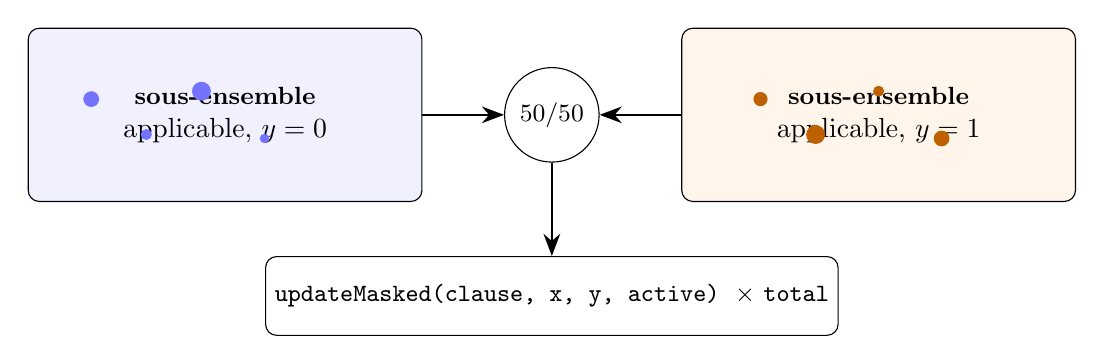
\begin{tikzpicture}
\node[draw, rounded corners, minimum width=5.0cm, minimum height=2.2cm, fill=blue!6, align=center] (c0) at (0,0)
     {\small\bfseries sous-ensemble\\applicable, $y=0$};
\foreach \x/\y/\r in {-1.7/0.2/0.10, -1.0/-0.25/0.07, -0.3/0.3/0.12, 0.5/-0.3/0.06}
  \fill[blue!55] (\x,\y) circle (\r);

\node[draw, rounded corners, minimum width=5.0cm, minimum height=2.2cm, fill=orange!8, align=center] (c1) at (8.3,0)
     {\small\bfseries sous-ensemble\\applicable, $y=1$};
\foreach \x/\y/\r in {6.8/0.2/0.09, 7.5/-0.25/0.12, 8.3/0.3/0.07, 9.1/-0.3/0.10}
  \fill[orange!75!black] (\x,\y) circle (\r);

\node[draw, circle, minimum size=1.2cm, fill=white] (coin) at (4.15,0) {\small 50/50};
\draw[-{Stealth[length=8pt]}, thick] (c0.east) -- (coin.west);
\draw[-{Stealth[length=8pt]}, thick] (c1.west) -- (coin.east);

\node[draw, rounded corners, minimum width=6.4cm, minimum height=1cm, font=\small] (upd) at (4.15,-2.3)
     {\code{updateMasked(clause, x, y, active)}\; $\times$ \code{total}};
\draw[-{Stealth[length=8pt]}, thick] (coin.south) -- (upd.north);
\end{tikzpicture}
\caption{Contrairement à l'ancienne architecture, le tirage se fait
\emph{exclusivement} à l'intérieur du sous-ensemble applicable de
\textbf{cette} clause --- jamais sur tout le dataset.}
\label{fig:sampler}
\end{figure}

% ======================================================
\section{Mesurer l'erreur, pondérer (AdaBoost par clause)}\label{sec:boost}
% ======================================================

Différence majeure avec l'ancienne architecture : l'erreur et la
repondération ne portent \textbf{que} sur le sous-ensemble applicable de la
clause --- les poids des exemples hors de ce sous-ensemble restent
\emph{inchangés} pour ce round.

\[
  \mathrm{err} = \frac{\displaystyle\sum_{i\,\in\,\text{applicable},\ \text{mal classé}} w_i}
  {\displaystyle\sum_{i\,\in\,\text{applicable}} w_i}
  \ \in\ [10^{-6},\,0.999],
  \qquad
  \alpha = \frac12\ln\!\left(\frac{1-\mathrm{err}}{\mathrm{err}}\right).
\]
\[
  w_i \mathrel{*}= \begin{cases} e^{\alpha} & \text{si } i \text{ applicable, mal classé} \\
                                  e^{-\alpha} & \text{si } i \text{ applicable, bien classé} \\
                                  1 & \text{si } i \text{ non applicable (inchangé)}\end{cases}
  \qquad\text{puis renormalise } \textstyle\sum_i w_i = 1.
\]

\begin{note}
Chaque clause est donc son \textbf{propre round de boosting complet}, et non
un composant d'un round partagé. Une clause chanceuse (tombée sur une bonne
combinaison de features) obtient un $\alpha$ élevé ; une clause malchanceuse
(condition sur des features non pertinentes) obtient $\alpha\approx0$ et pèse
presque rien dans le vote final --- sans jamais perturber les poids des
exemples hors de son sous-ensemble.
\end{note}

% ======================================================
\section{Combiner les $M$ clauses et décider}\label{sec:combine}
% ======================================================

\[
  \mathrm{score}(x) = \sum_{\substack{m=1 \\ \code{applies}_m(x) \,\wedge\, \neg\code{isEmpty}_m}}^{M}
  \alpha_m \cdot \big(2\cdot C_m(x) - 1\big),
  \qquad
  \hat y = \begin{cases}1 & \text{si } \mathrm{score}(x) > 0\\ 0 & \text{sinon.}\end{cases}
\]

\begin{figure}[h]
\centering
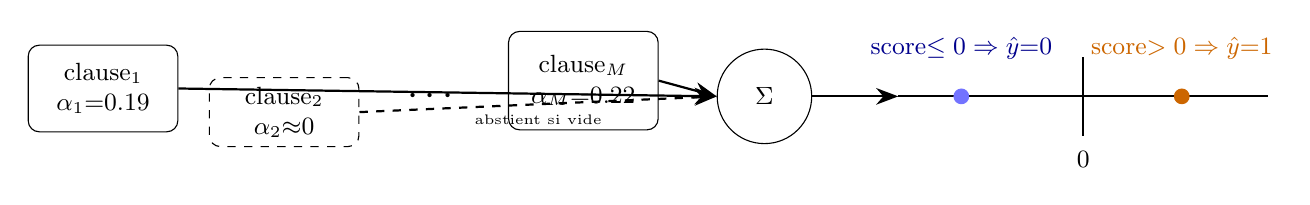
\begin{tikzpicture}
\node[draw, rounded corners, minimum width=1.9cm, minimum height=1.1cm, font=\small, align=center] (n1) at (0,0.4) {clause$_1$\\$\alpha_1{=}0.19$};
\node[draw, rounded corners, minimum width=1.9cm, minimum height=0.7cm, font=\small, align=center, dashed] (n2) at (2.3,0.1) {clause$_2$\\$\alpha_2{\approx}0$};
\node[font=\Large] at (4.2,0.3) {$\cdots$};
\node[draw, rounded corners, minimum width=1.9cm, minimum height=1.25cm, font=\small, align=center] (nM) at (6.1,0.5) {clause$_M$\\$\alpha_M{=}0.22$};

\node[draw, circle, minimum size=1.2cm, font=\small] (sum) at (8.4,0.3) {$\Sigma$};
\draw[-{Stealth[length=8pt]}, thick] (n1.east) -- (sum.west);
\draw[-{Stealth[length=8pt]}, thick, dashed] (n2.east) -- (sum.west) node[midway,below,font=\tiny] {abstient si vide};
\draw[-{Stealth[length=8pt]}, thick] (nM.east) -- (sum.west);

\draw[-{Stealth[length=8pt]}, thick] (sum.east) -- (10.1,0.3);
\draw[thick] (10.1,0.3) -- (14.8,0.3);
\draw[thick] (12.45,-0.2) -- (12.45,0.8);
\node[font=\small] at (12.45,-0.5) {0};
\fill[blue!55] (10.9,0.3) circle (0.1);
\node[font=\small, blue!55!black, above] at (10.9,0.65) {score$\le0\Rightarrow\hat y{=}0$};
\fill[orange!80!black] (13.7,0.3) circle (0.1);
\node[font=\small, orange!80!black, above] at (13.7,0.65) {score$>0\Rightarrow\hat y{=}1$};
\end{tikzpicture}
\caption{Vote pondéré final. Les clauses non applicables à $x$, ou vides,
\textbf{n'entrent pas dans la somme} (représentées en pointillé) --- elles ne
votent ni pour $0$ ni pour $1$, elles s'abstiennent purement et simplement.}
\label{fig:combine}
\end{figure}

\subsection{Extension multi-classe (one-vs-rest)}

Pour Iris, Digits et MNIST : un ensemble \emph{indépendant} de $M$ clauses par
classe $c$, entraîné avec l'étiquette relabellisée $y'=\mathbb{1}[y=c]$.

\[
  \hat y = \operatorname*{argmax}_{c\,\in\,\{1,\dots,\text{numClasses}\}} \mathrm{score}_c(x).
\]

Chaque classe a son propre ensemble de clauses, ses propres tirages de
conditionnement, ses propres $\alpha$ --- aucun partage entre classes.

% ======================================================
\section{Hyperparamètres et meilleures configurations trouvées}
% ======================================================

\begin{center}
\renewcommand{\arraystretch}{1.3}
\begin{tabular}{lll}
\toprule
Paramètre & Contrôle & Ce qu'on a appris \\
\midrule
$M$ & nombre de clauses & compense la loterie combinatoire ($\binom{n}{K}$) \\
$K$ & features conditionnées / clause & $K{=}1$ suffit si $n$ petit ; $K$ plus grand débloque des gains si $M$ suit \\
$S\in[0,1]$ & proba.\ de mouvement vers \Inc & probabilité réelle --- $S{=}1$ quasi toujours optimal \\
$\alpha\in[0,1]$ & proba.\ de mouvement vers \Exc & optimum dataset-dépendant, trouvé par balayage \\
$N$ & demi-plage d'états & trop grand + \code{total} fixe $\Rightarrow$ jamais saturé à temps \\
\code{total} & tirages d'entraînement / clause & doit rester assez petit pour ne pas saturer aveuglément $S,\alpha$ \\
\bottomrule
\end{tabular}
\end{center}

\vspace{0.6em}

\begin{center}
\renewcommand{\arraystretch}{1.3}
\begin{tabular}{lccccccc}
\toprule
Dataset & $M$ & $K$ & $S$ & $\alpha$ & $N$ & \code{total} & Accuracy (20 runs) \\
\midrule
XOR      & 200  & 1 & 1.0 & 0.35 & 50  & 1500  & $99.07\%\pm2.16\%$ \\
Iris     & 1500 & 2 & 1.0 & 0.30 & 100 & 20000 & $95.5\%\pm4.25\%$ \\
Mux11    & 8000 & 3 & 1.0 & 0.30 & 100 & 20000 & $99.97\%\pm0.02\%$ \\
Parity3  & 1000 & 2 & 1.0 & 0.30 & 100 & 20000 & $91.9\%\pm7.4\%$ \\
Digits   & 300  & 1 & 1.0 & 0.30 & 100 & 20000 & $92.3$--$92.6\%$ (K=2 en cours) \\
MNIST    & 40000 & 1 & 1.0 & 0.30 & 256 & 20000 & $90.3\%$ (budget complet du papier) \\
\bottomrule
\end{tabular}
\end{center}

\vfill
\hrule
\vspace{0.4em}
\noindent\footnotesize
\textbf{Portée} : \code{random\_stump\_perclause\_boost.cpp} $\cdot$
\code{random\_stump\_multifeature.cpp} $\cdot$
\code{random\_stump\_multiclass.cpp} $\cdot$
\code{random\_stump\_multifeature\_multiclass.cpp} --- tous réutilisant
\code{Clause} et \code{updateMasked} de \texttt{tsetlin\_engine.h}. Appliqué
identiquement aux six datasets. Contrairement à \emph{anatomie\_moteur.tex}
(architecture précédente), \textbf{aucun routeur, à aucun niveau}.

\end{document}
